\section{Experimentation}
\label{sec:experimentation}
\subsection{First experiment}
The goal of the first experiment is to apply EM and DBSCAN to the generated data with blob shape, i.e. to sub-figures \ref{subfig:4-4-truth}, \ref{subfig:7-3-truth}, \ref{subfig:30-30-truth} and \ref{subfig:30-30-6-truth}.

\begin{figure*}[t!]
    \begin{subfigure}[b]{0.45\textwidth}
        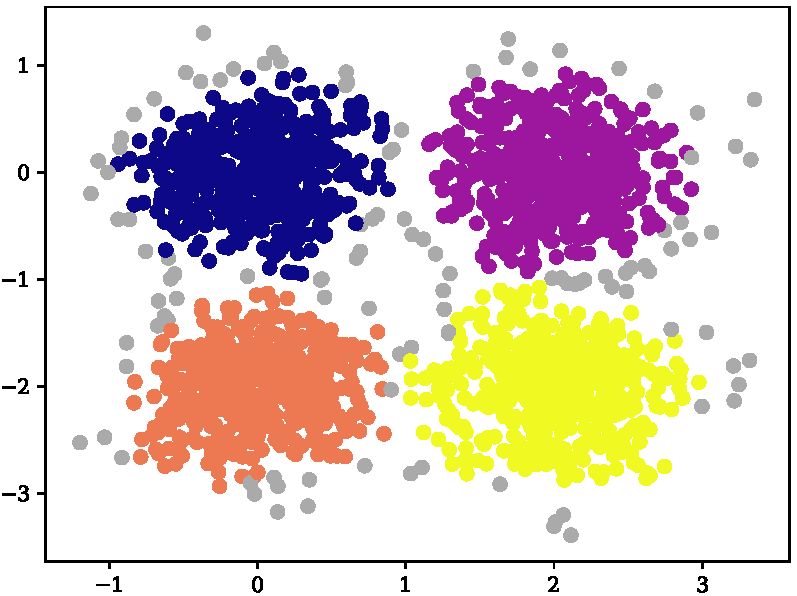
\includegraphics[width=\textwidth]{../plots/4-4_pred_dbscan.pdf}
        \caption{DBSCAN}
        \label{subfig:4-4-dbscan}
    \end{subfigure}
    \hspace{0.09\textwidth}
    \begin{subfigure}[b]{0.45\textwidth}
            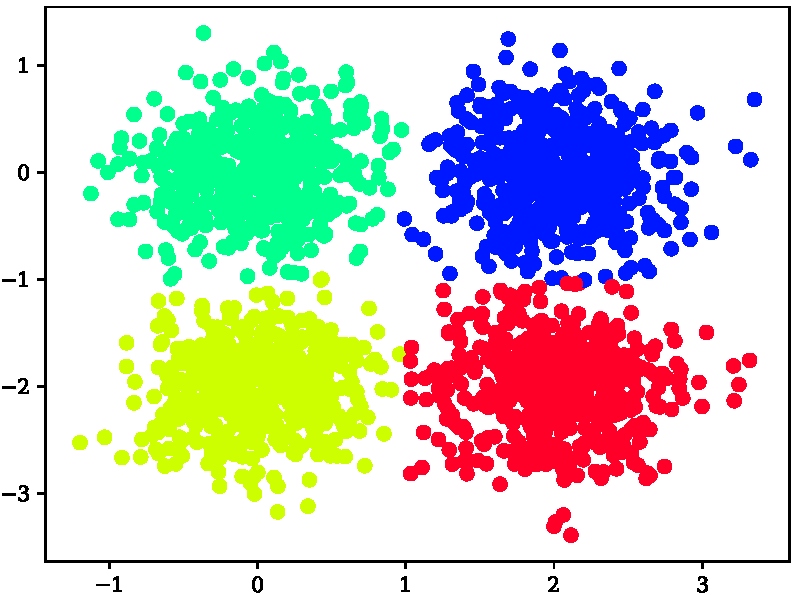
\includegraphics[width=\textwidth]{../plots/4-4_pred_em.pdf}
            \caption{EM}
            \label{subfig:4-4-em}
    \end{subfigure}
\end{figure*}
\begin{figure*}[t!]
    \begin{subfigure}[b]{0.45\textwidth}
        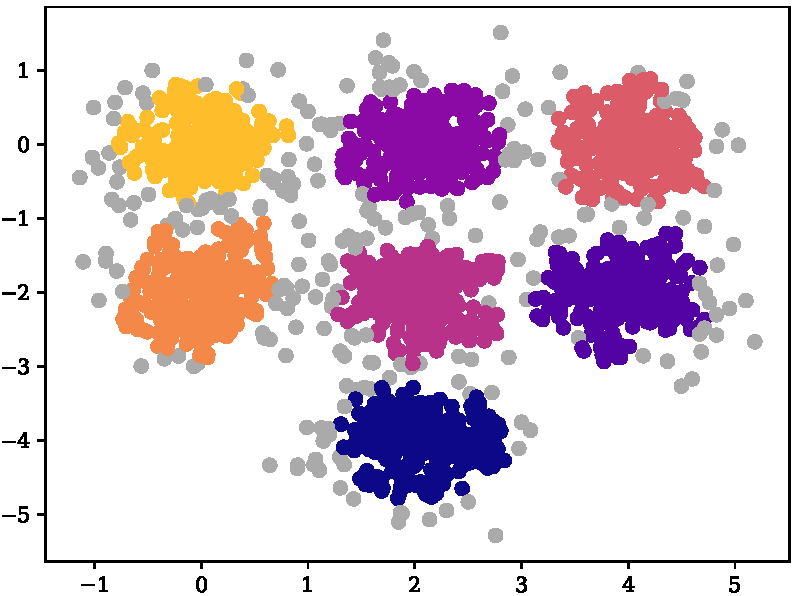
\includegraphics[width=\textwidth]{../plots/7-3_pred_dbscan.pdf}
        \caption{DBSCAN}
        \label{subfig:7-3-dbscan}
    \end{subfigure}
    \hspace{0.09\textwidth}
    \begin{subfigure}[b]{0.45\textwidth}
        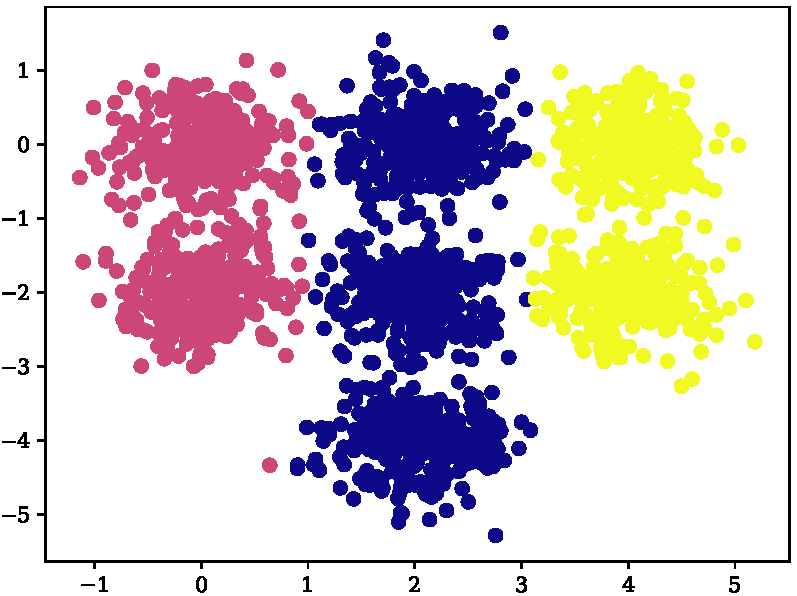
\includegraphics[width=\textwidth]{../plots/7-3_pred_em.pdf}
        \caption{EM}
        \label{subfig:7-3-em}
    \end{subfigure}
\end{figure*}
\begin{figure*}[t!]
    \begin{subfigure}[b]{0.45\textwidth}
        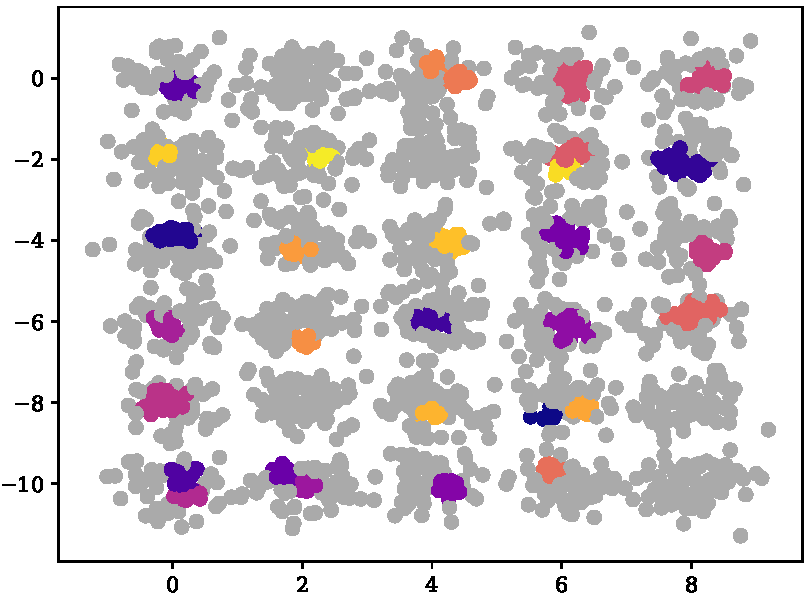
\includegraphics[width=\textwidth]{../plots/30-30_pred_dbscan.pdf}
        \caption{DBSCAN}
        \label{subfig:30-30-dbscan}
    \end{subfigure}
    \hspace{0.09\textwidth}
    \begin{subfigure}[b]{0.45\textwidth}
        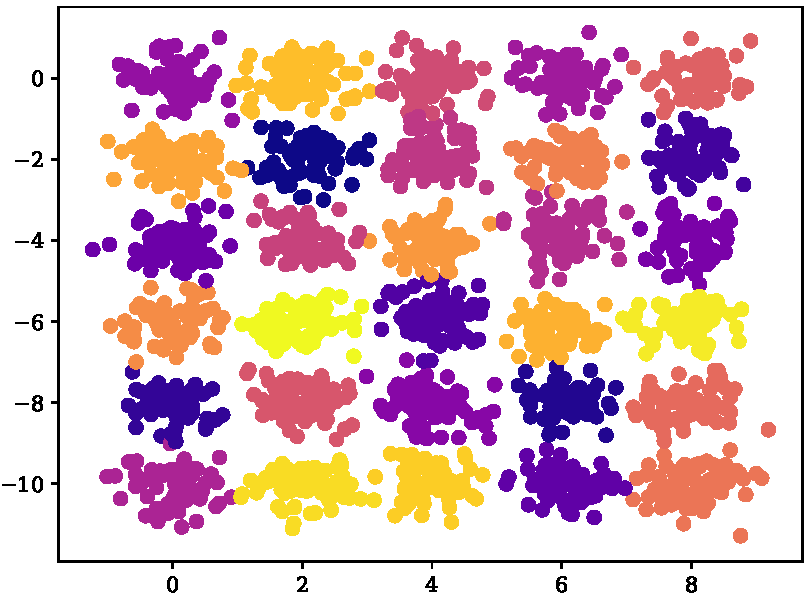
\includegraphics[width=\textwidth]{../plots/30-30_pred_em.pdf}
        \caption{EM}
        \label{subfig:30-30-em}
    \end{subfigure}
\end{figure*}
\begin{figure*}[t!]
    \begin{subfigure}[b]{0.45\textwidth}
        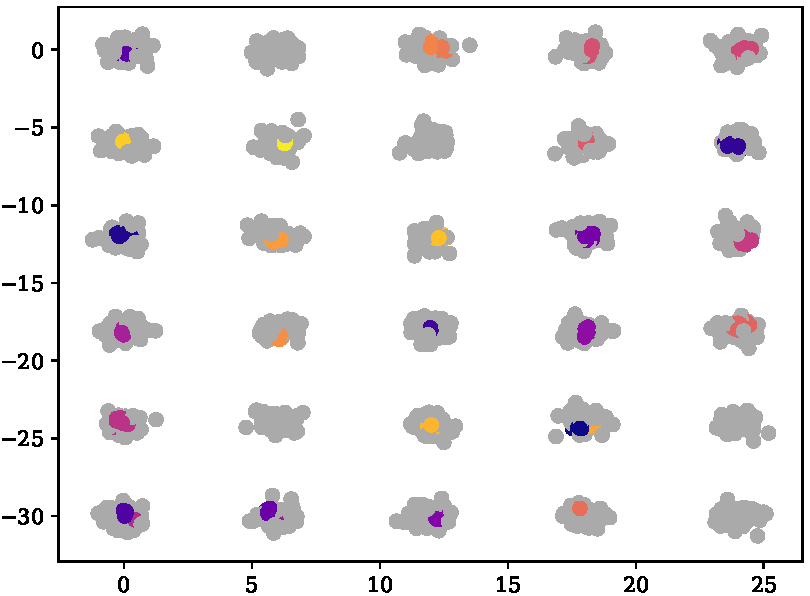
\includegraphics[width=\textwidth]{../plots/30-30-6_pred_dbscan.pdf}
        \caption{DBSCAN}
        \label{subfig:30-30-6-dbscan}
    \end{subfigure}
    \hspace{0.09\textwidth}
    \begin{subfigure}[b]{0.45\textwidth}
        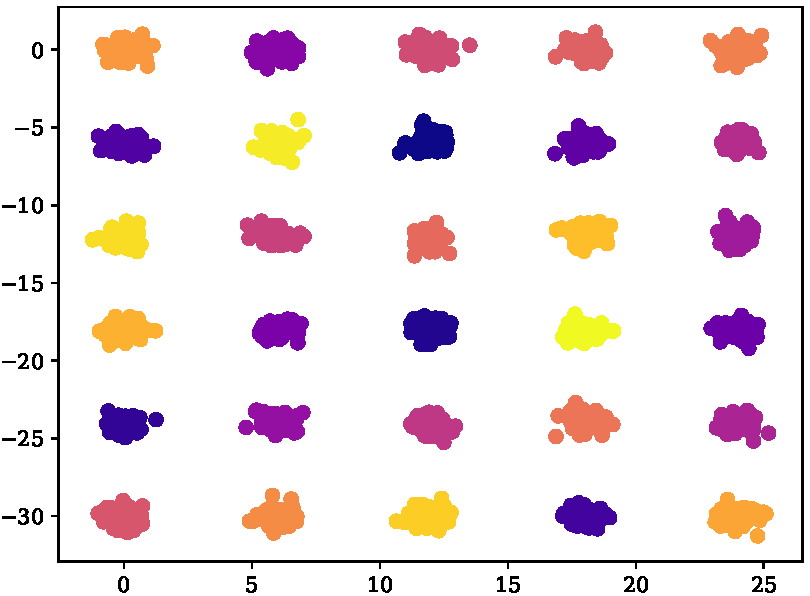
\includegraphics[width=\textwidth]{../plots/30-30-6_pred_em.pdf}
        \caption{EM}
        \label{subfig:30-30-6-em}
    \end{subfigure}
\end{figure*}
\begin{figure*}[t!]
    \begin{subfigure}[b]{0.45\textwidth}
        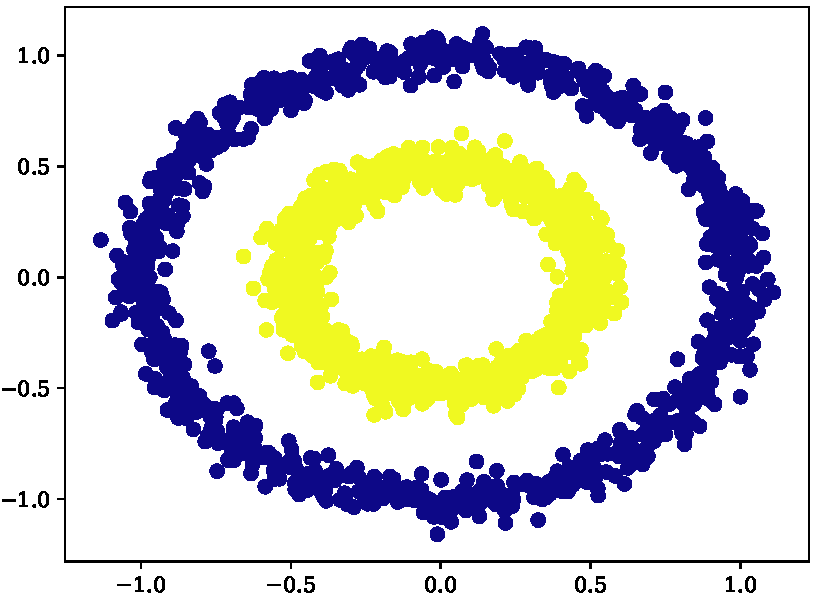
\includegraphics[width=\textwidth]{../plots/circle_dbscan.pdf}
        \caption{DBSCAN}
        \label{subfig:circle-dbscan}
    \end{subfigure}
    \hspace{0.09\textwidth}
    \begin{subfigure}[b]{0.45\textwidth}
        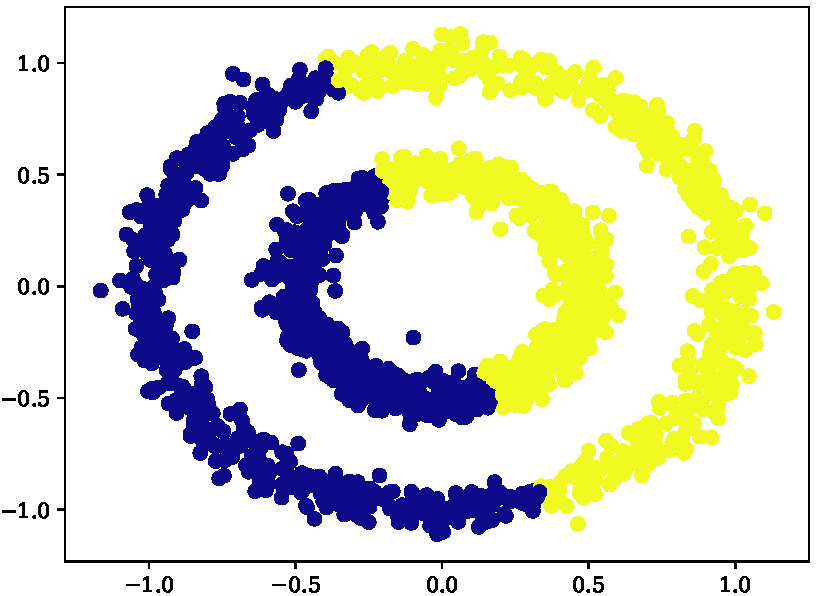
\includegraphics[width=\textwidth]{../plots/circle_em.pdf}
        \caption{EM}
        \label{subfig:circle-em}
    \end{subfigure}
\end{figure*}
\begin{figure*}[t!]
    \begin{subfigure}[b]{0.45\textwidth}
        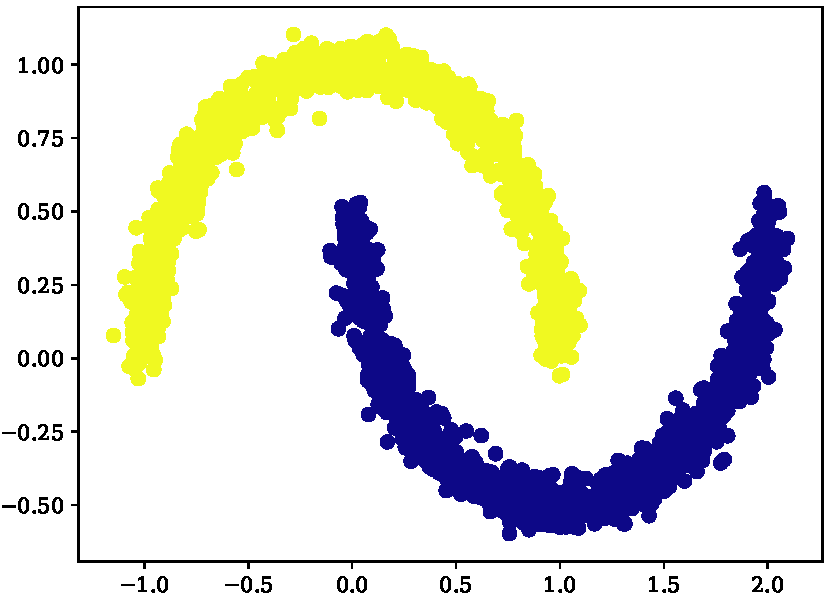
\includegraphics[width=\textwidth]{../plots/moons_dbscan.pdf}
        \caption{DBSCAN}
        \label{subfig:moon-dbscan}
    \end{subfigure}
    \hspace{0.09\textwidth}
    \begin{subfigure}[b]{0.45\textwidth}
        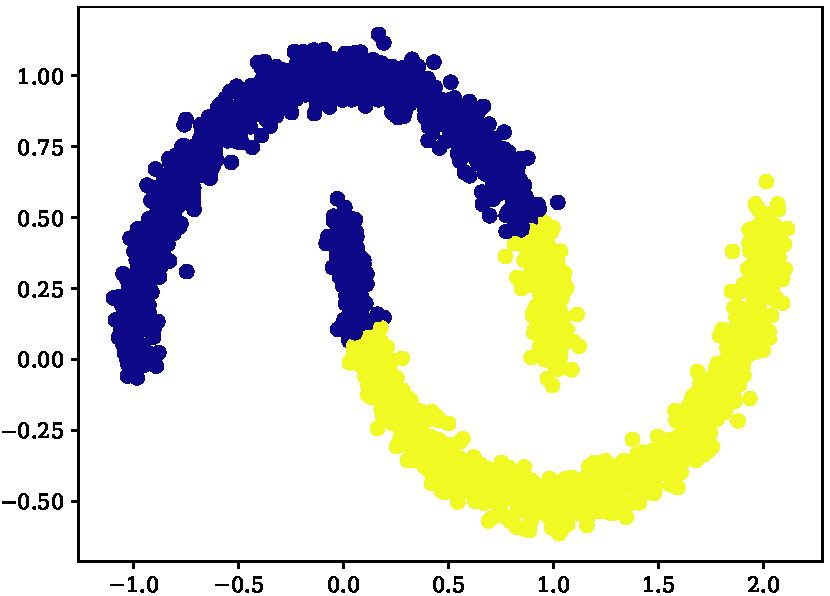
\includegraphics[width=\textwidth]{../plots/moons_em.pdf}
        \caption{EM}
        \label{subfig:moon-em}
    \end{subfigure}
\end{figure*}
